\section{Doménový model}
%%%%%%%%%%%%%%%%%%%%%%%%%%%%
Ze schůze s majitelem a poskytnuté excelové tabulky byly identifikovány entity figurující v chodu pneuservisu. Podle tohoto byl nejdříve zmapován současný stav, a poté byl vytvořen návrh budoucího stavu systému.

Poskytnutá excelová tabulka obsahuje data, která pneuservis nyní sbírá. Ta se dají rozdělit do následujících kategorií:
\begin{description}
    \item [Zákaznická data] poskytují informace o zákazníkovi: jméno, telefon, email, adresa\dots
    \item [Data vozidel] poskytují informace o vozidle: SPZ, výrobce, model\dots
    \item [Data disků a pneumatik] poskytují informace o discích a pneumatikách: značka, poškození\dots
    \item [Data služeb] poskytují informace o provedených službách přezutí, mytí, oprav a uskladnění.
\end{description}
%%%%%%%%%%%%%%%%%%%%%%%%%%%%
\subsection{Současný stav}
Administrátor pneuservisu registruje zákazníky, jejich automobily a sady pneumatik/kol.

Klíčovou entitou jsou sady pneumatik/kol. Sady nejsou rozděleny do dvou rozdílných entit, protože administrace pneuservisu je vnímá jako jednu entitu, která se liší pouze v parametru určujícím, zda se jedná o pneumatiky nebo kola. Na tomto místě je dobré si uvědomit rozdíl mezi diskem, pneumatikou a kolem (kolo se skládá z disku a pneumatiky).

Dále administrátor pneuservisu vytváří rezervace automobilů k přezutí pneumatik/kol. 

Model současné situace je vidět na obrázku \ref{fig:Domain_model_-_old}. Tento stav má své nedostatky, například: 
\begin{itemize}
    \item Sady kol a pneumatik jsou považovány za jeden objekt a nemají žádný identifikátor. 
    \item Mytí, opravy a uskladnění nejsou samostatné entity. 
    \item Rezervacím chybí nějaký identifikátor.
\end{itemize}

Z těchto nedostatků je jasné, že model současného stavu je odrazem způsobu, jakým majitel informace zapisuje. Pro obecné použití je tento model nevhodný, a proto je potřeba zvolit komplexnější řešení.
\begin{figure}[h!]
    \centering
    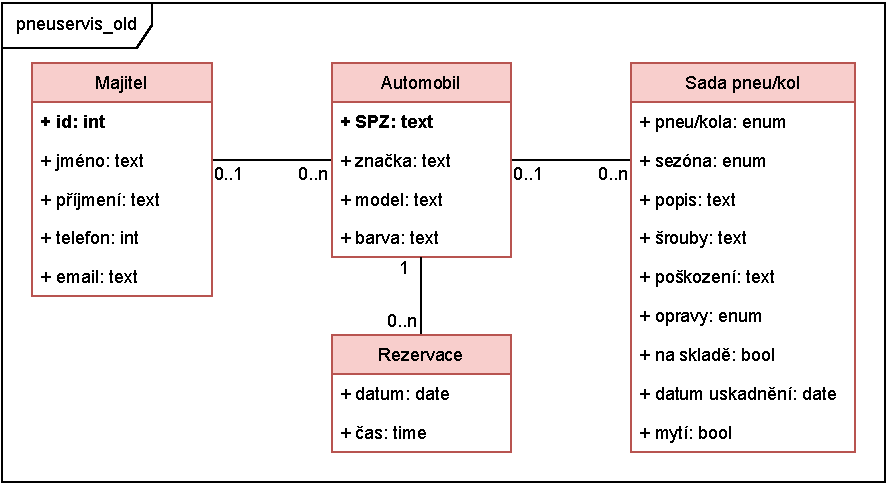
\includegraphics[width=0.8\textwidth]{assets/6_návrh/Domain model-Old.drawio.pdf}
    \caption{Doménový model -- současný stav.}
    \label{fig:Domain_model_-_old}
\end{figure}
\FloatBarrier
%%%%%%%%%%%%%%%%%%%%%%%%%%%%
\subsection{Budoucí stav}
Model současného stavu je dobrým odrazovým můstkem pro komplexnější systém podporující agendu pneuservisu. 

Díky přechodu na novou platformu je možné model budoucího stavu vytvořit od základů \uv{na zelené louce}.

Model budoucího stavu byl vytvořen s ohledem na technologická omezení platformy Salesforce. Mezi tato omezení patří například: 
\begin{itemize}
    \item Systém podporuje pouze 1:N relace.
    \item Existují dva druhy relací, silná a slabá. Silná relace je vnímána mezi objekty jako vztah rodič--potomek.
    \item Každý objekt musí mít jméno které hraje roli identifikátoru, ale nemusí být unikátní.
    \item Platforma Salesforce poskytuje vlastní standardní datové typy pro řadu atributů. Příkladem je atribut \emph{datum} a datový typ \emph{Date}, který vytvoří textové pole s kalendářem pro vložení data.
\end{itemize}

Model budoucího stavu zahrnuje rozdělení sad pneumatik/kol na entity \emph{Disky} a \emph{Pneumatiky}. To dává administrátorům pneuservisu svobodu zaznamenávat situace:
\begin{itemize}
    \item zákazník chce vyměnit pouze disky,
    \item zákazník chce vyměnit pouze pneumatiky,
    \item zákazník chce kompletně vyměnit kola.
\end{itemize}

Vylepšení která systém přináší jsou odrazem přidaných entit.

Do tohoto modelu byly přidány služby, které pneuservis poskytuje. Tabulky \emph{Oprava}, \emph{Mytí}, \emph{Uskladnění} a \emph{Přezutí} hrají roli vazební tabulky pro M:N vazbu mezi jednotlivými typy služeb a zákazníky. Tyto tabulky slouží jako evidence všech objednaných služeb.

V modelu figurují i tabulky \emph{Typ opravy}, \emph{Typ mytí}, a \emph{Typ přezutí}, které umožňují administrátorovi pneuservisu nastavit typy služeb a jejich ceny.

Oproti modelu současného stavu se jedná o obecné a komplexní řešení, které je možné využít i u jiných pneuservisů.

Celkové schéma modelu je vidět na obrázku \ref{fig:Domain_model_-_new}.

O tento model se v další kapitole opírá implementace systému na platformě Salesforce.

\begin{sidewaysfigure}[h!]
    \centering
    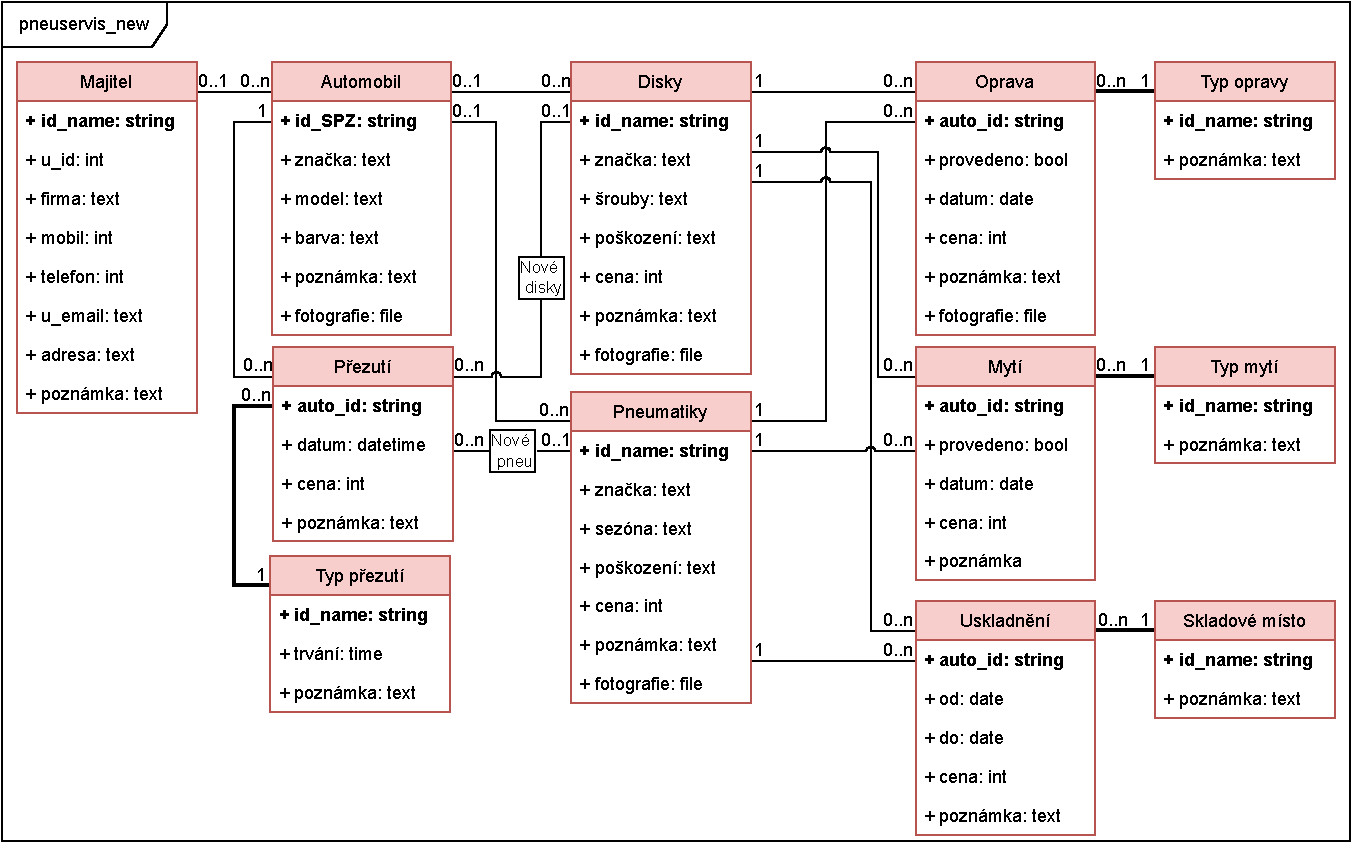
\includegraphics[width=\textwidth]{assets/6_návrh/Domain model-New.drawio.pdf}
    \caption{Doménový model -- budoucí stav.}
    \label{fig:Domain_model_-_new}
\end{sidewaysfigure}
